%! Author = Len Washington III
%! Date = 11/6/24

% Preamble
\documentclass[
	chapter=8,
	title={Periodic Properties of the Elements},
	showanswers=true,
]{chem122notes}

% Packages

% Document
\begin{document}

\section{Outline}\label{sec:outline-8}
\begin{itemize}
	\item History of the periodic table
	\item Effective nuclear charge
	\item Sizes of atoms and ions
	\item Trends in ionization energies
	\item Trends in electron affinities
\end{itemize}

\begin{figure}[H]
	\centering
	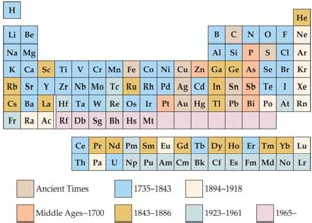
\includegraphics[width=\textwidth]{chapter8/periodic-table-dates}
	\caption{Discovery Dates of the Elements}
	\label{fig:periodic-table-dates}
\end{figure}

\section{Development of the Periodic Table}\label{sec:development-of-the-periodic-table}
\begin{itemize}
	\item Mendeleev's insistence that elements with similar properties be listed in the same group lead him to leave several blanks in the periodic table.
	\item For example, Mendeleev predicted some properties of now what is called Germanium based on the fact that it is in the same group as Silicon.
	Silicon was discovered almost 100 years before that of Germanium!
	\item Once germanium was discovered, its observed properties matched exceptionally well with Mendeleev's predictions (see the table on the next slide).
\end{itemize}

\begin{table}[H]
	\centering
	\caption{Comparison of the Properties of Eka-Silicon (\emph{``under'' silicon}) Predicted by Mendeleev with the Observed Properties of Germanium}
	\label{tab:silicon-properties}
	\begin{tabular}{*{3}{p{0.3\textwidth}}}
		\textbf{Property} & \textbf{Mendeleev's Predictions for Eka-Silicon (made in 1871)} & \textbf{Observed Properties of Germanium (discovered in 1886)}\\
		\hline
		Atomic weight & 72 & 72.59\\
		Density (g/$\mbox{cm}^{3}$) & 5.5 & 5.35\\
		Specific heat (J/g$\times$K) & 0.305 & 0.309\\
		Melting point (\textdegree{}C) & High & 947\\
		Color & Dark gray & Grayish white\\
		Formula of oxide & \ce{XO2} & \ce{GeO2}\\
		Density of oxide (g/$\mbox{cm}^{3}$) & 4.7 & 4.70\\
		Formula of chloride & \ce{XCl4} & \ce{GeCl4}\\
		Boiling point of chloride (\textdegree{}C) & A little under 100 & 84\\
		\hline
	\end{tabular}
\end{table}

\definition{Periodic law 1860--1870's (Mendeleev and Meyer)}{\emph{A periodic repetition of physical and chemical properties} occurs when the elements are arranged in order of increasing atomic \textit{weight [\emph{number}]}}

\begin{figure}[H]
	\centering
	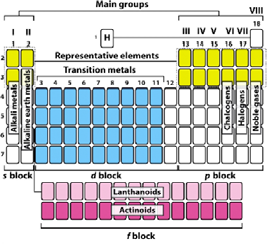
\includegraphics[width=\textwidth]{chapter8/periodic-table-2}
	\caption{}
	\label{fig:periodic-table-2}
\end{figure}

\section{Ordering by Atomic Weight}\label{sec:ordering-by-atomic-weight}
\textbf{Inconsistencies in ordering by atomic weight:}
\begin{itemize}\newcommand{\weights}[3]{\ce{#1} (#2 amu; $Z=#3$)}
	\item \weights{Co}{58.93}{27} and \weights{Ni}{58.69}{28}
	\item \weights{Ar}{39.95}{18} and \weights{K}{39.10}{19}
	\item \weights{Te}{127.60}{52} and \weights{I}{126.90}{53}
\end{itemize}
\emph{However, all of the above are correctly ordered by atomic number, $Z$ (i.e., the number of protons).}

\section{Development of Periodic Table}\label{sec:development-of-periodic-table}
\begin{itemize}
	\item Elements in the same group generally have similar chemical properties.
	\item However, physical properties are not necessarily similar.
	\item For example, even though Oxygen and Sulfur are in the same group (6A), Oxygen is a colorless gas, while Sulfur is a yellow solid under normal conditions.
\end{itemize}

\section{But why do elements in the same group have similar properties?}\label{sec:but-why-do-elements-in-the-same-group-have-similar-properties?}




\section{Trends in First Ionization Energies}\label{sec:trends-in-first-ionization-energies}
\begin{itemize}
	\item As one goes down a group, less energy is required to remove the first electron.
	\begin{itemize}
		\item For atoms in the same group, $Z_{eff}$ is essentially the same, but the valence electrons are farther from than $\dots$
	\end{itemize}
	\item Generally, as one goes across a row/period, it becomes more difficult to remove an electron.
	\begin{itemize}
		\item As you go from left to right $\rightarrow Z_{eff}$ increases!
	\end{itemize}
\end{itemize}

Account for the decrease in ionization energy in going from nitrogen (N) to oxygen (O) despite the increase in effective nuclear charge ($Z_{eff}$).

\begin{answer}
\end{answer}

\section{Electron Affinity}\label{sec:electron-affinity}
Electron affinity is the energy change accompanying the addition of an electron to a gaseous atom:
\begin{equation*}
\begin{aligned}
	\ce{CL(g) + e- ->  Cl-(g)}\ \ \ \ \ E_{a} = -349 \frac{\mbox{kJ}}{\mbox{mol}}
\end{aligned}
\end{equation*}
Energy is typically released when an electron is added to a gaseous atom.
The process is said to be \emph{exothermic}, so the energy has a negative sign associated with it.\\

The electron affinity of lithium is a negative value, whereas the electron affinity of Beryllium is a positive value.
Use electron configuration to account for this observation.

\end{document}
